% v2-acmsmall-sample.tex, dated March 6 2012
% This is a sample file for ACM small trim journals
%
% Compilation using 'acmsmall.cls' - version 1.3 (March 2012), Aptara Inc.
% (c) 2010 Association for Computing Machinery (ACM)
%
% Questions/Suggestions/Feedback should be addressed to => "acmtexsupport@aptaracorp.com".
% Users can also go through the FAQs available on the journal's submission webpage.
%
% Steps to compile: latex, bibtex, latex latex
%
% For tracking purposes => this is v1.3 - March 2012

\documentclass[prodmode,acmtecs]{acmsmall} % Aptara syntax


% Package to generate and customize Algorithm as per ACM style
\usepackage[ruled]{algorithm2e}
\renewcommand{\algorithmcfname}{ALGORITHM}
\SetAlFnt{\small}
\SetAlCapFnt{\small}
\SetAlCapNameFnt{\small}
\SetAlCapHSkip{0pt}
\IncMargin{-\parindent}

% Metadata Information
% \acmVolume{9}
% \acmNumber{4}
% \acmArticle{39}
% \acmYear{2010}
% \acmMonth{3}

% Copyright
%\setcopyright{acmcopyright}
%\setcopyright{acmlicensed}
%\setcopyright{rightsretained}
%\setcopyright{usgov}
%\setcopyright{usgovmixed}
%\setcopyright{cagov}
%\setcopyright{cagovmixed}

% DOI
% \doi{0000001.0000001}

%ISSN
% \issn{1234-56789}

% Document starts
\begin{document}

% Page heads
\markboth{Y. Xie et al.}{Ranking Code Completion Candidates}

% Title portion
\title{Ranking Code Completion Candidates}
\author{Yanan Xie
\affil{yaxie@ucsc.edu}
Yifei Wu
\affil{ywu151@ucsc.edu}
Ziyi Chen
\affil{zchen139@ucsc.edu}
}

\begin{abstract}
Multifrequency media access control has been well understood in
general wireless ad hoc networks, while in wireless sensor networks,
researchers still focus on single frequency solutions. In wireless
sensor networks, each device is typically equipped with a single
radio transceiver and applications adopt much smaller packet sizes
compared to those in general wireless ad hoc networks. Hence, the
multifrequency MAC protocols proposed for general wireless ad hoc
networks are not suitable for wireless sensor network applications,
which we further demonstrate through our simulation experiments. In
this article, we propose MMSN, which takes advantage of
multifrequency availability while, at the same time, takes into
consideration the restrictions of wireless sensor networks. Through
extensive experiments, MMSN exhibits the prominent ability to utilize
parallel transmissions among neighboring nodes. When multiple physical
frequencies are available, it also achieves increased energy
efficiency, demonstrating the ability to work against radio
interference and the tolerance to a wide range of measured time
synchronization errors.
\end{abstract}


\maketitle


\section{Introduction}

\begin{figure}
\centerline{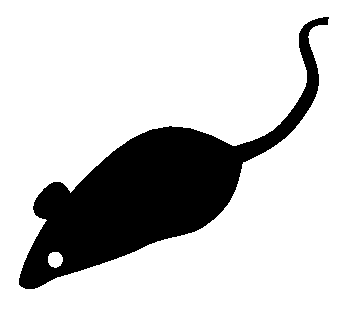
\includegraphics{acmsmall-mouse}}
\caption{Code before preprocessing.}
\label{fig:one}
\end{figure}

\begin{table}%
\tbl{Simulation Configuration\label{tab:one}}{%
\begin{tabular}{|l|l|}
\hline
TERRAIN{$^a$}   & (200m$\times$200m) Square\\\hline
Node Number     & 289\\\hline
Node Placement  & Uniform\\\hline
Application     & Many-to-Many/Gossip CBR Streams\\\hline
Payload Size    & 32 bytes\\\hline
Routing Layer   & GF\\\hline
MAC Layer       & CSMA/MMSN\\\hline
Radio Layer     & RADIO-ACCNOISE\\\hline
Radio Bandwidth & 250Kbps\\\hline
Radio Range     & 20m--45m\\\hline
\end{tabular}}
\begin{tabnote}%
\Note{Source:}{This is a table
sourcenote. This is a table sourcenote. This is a table
sourcenote.}
\vskip2pt
\Note{Note:}{This is a table footnote.}
\tabnoteentry{$^a$}{This is a table footnote. This is a
table footnote. This is a table footnote.}
\end{tabnote}%
\end{table}%

\section{Conclusions}

In this article, we develop the first multifrequency MAC protocol for
WSN applications in which each device adopts a
single radio transceiver. The different MAC design requirements for
WSNs and general wireless ad-hoc networks are
compared, and a complete WSN multifrequency MAC design (MMSN) is
put forth. During the MMSN design, we analyze and evaluate different
choices for frequency assignments and also discuss the nonuniform
back-off algorithms for the slotted media access design.

% Start of "Sample References" section

\section{Typical references in new ACM Reference Format}
A paginated journal article \cite{Abril07},


% Acknowledgments
\begin{acks}
The authors would like to thank Dr. Maura Turolla of Telecom
Italia for providing specifications about the application scenario.
\end{acks}

% Bibliography
\bibliographystyle{ACM-Reference-Format-Journals}
\bibliography{acmsmall-sample-bibfile}
 


\end{document}
% End of v2-acmsmall-sample.tex (March 2012) - Gerry Murray, ACM


